
  \subsubsection{Front-end}
  \paragraph{Informazioni sul package}
    \begin{figure}[H] 
      \begin{center}
        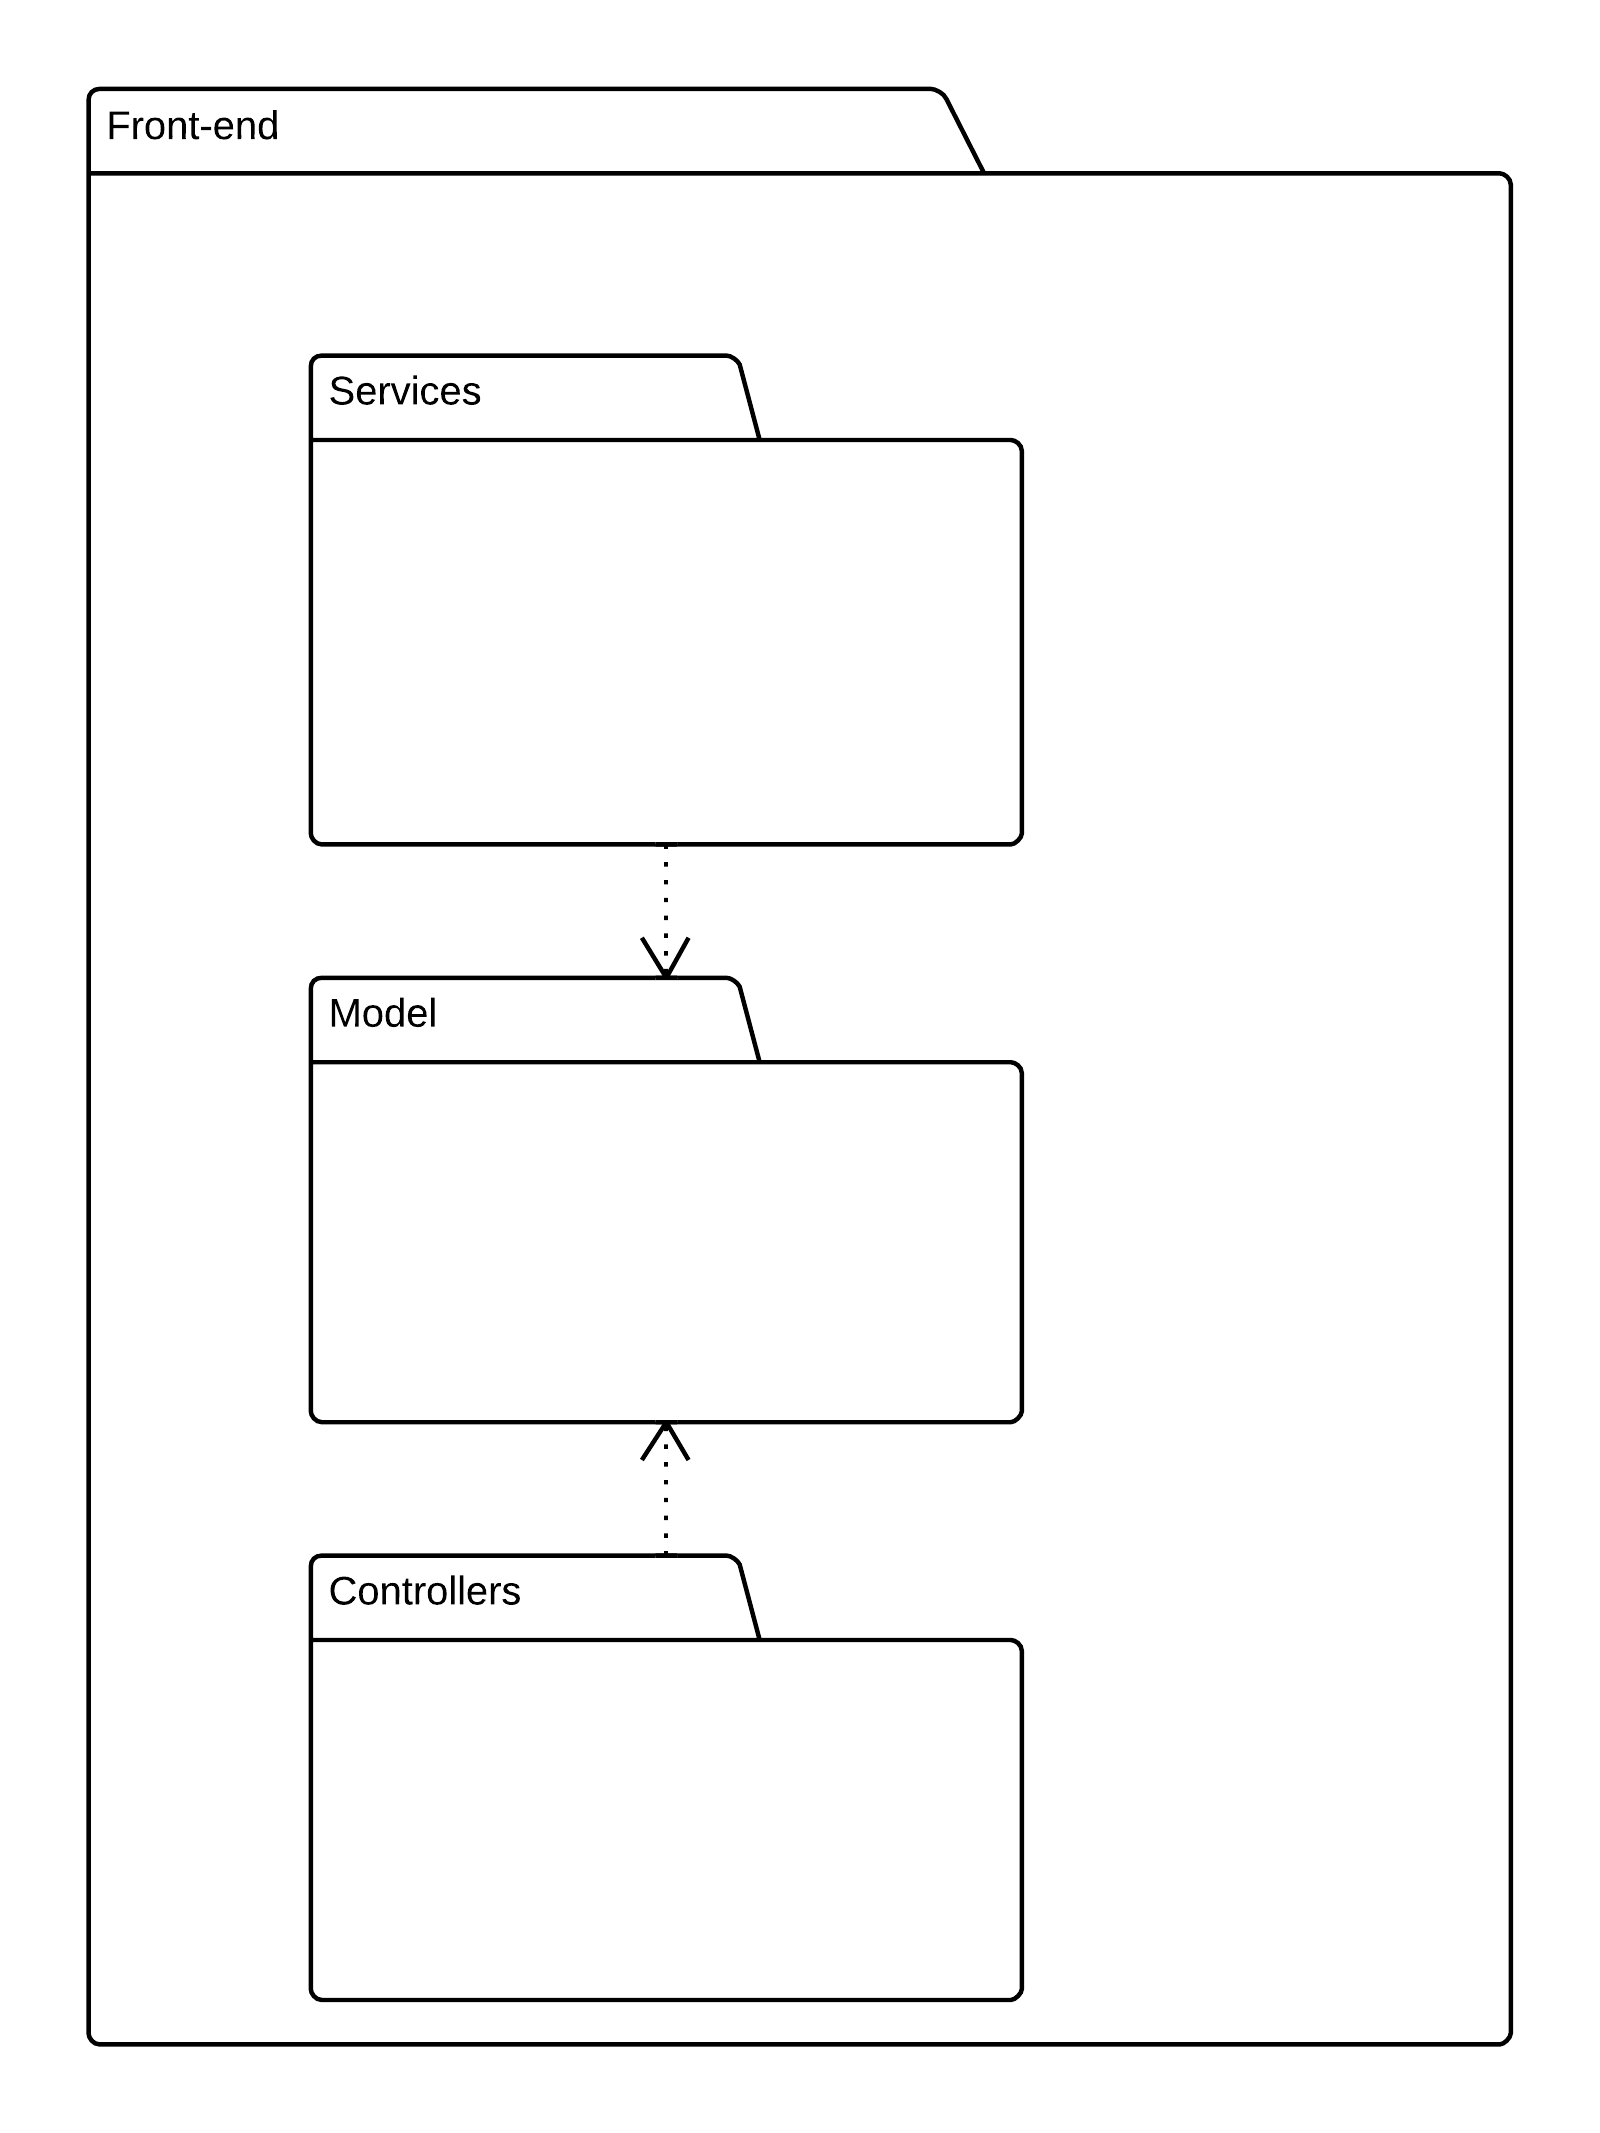
\includegraphics[width=\textwidth]{uml/package/Front-end.png}
        \caption{Diagramma packages Front-end}
      \end{center}  
    \end{figure} 
    
   \begin{figure}[H] 
      \begin{center} 
        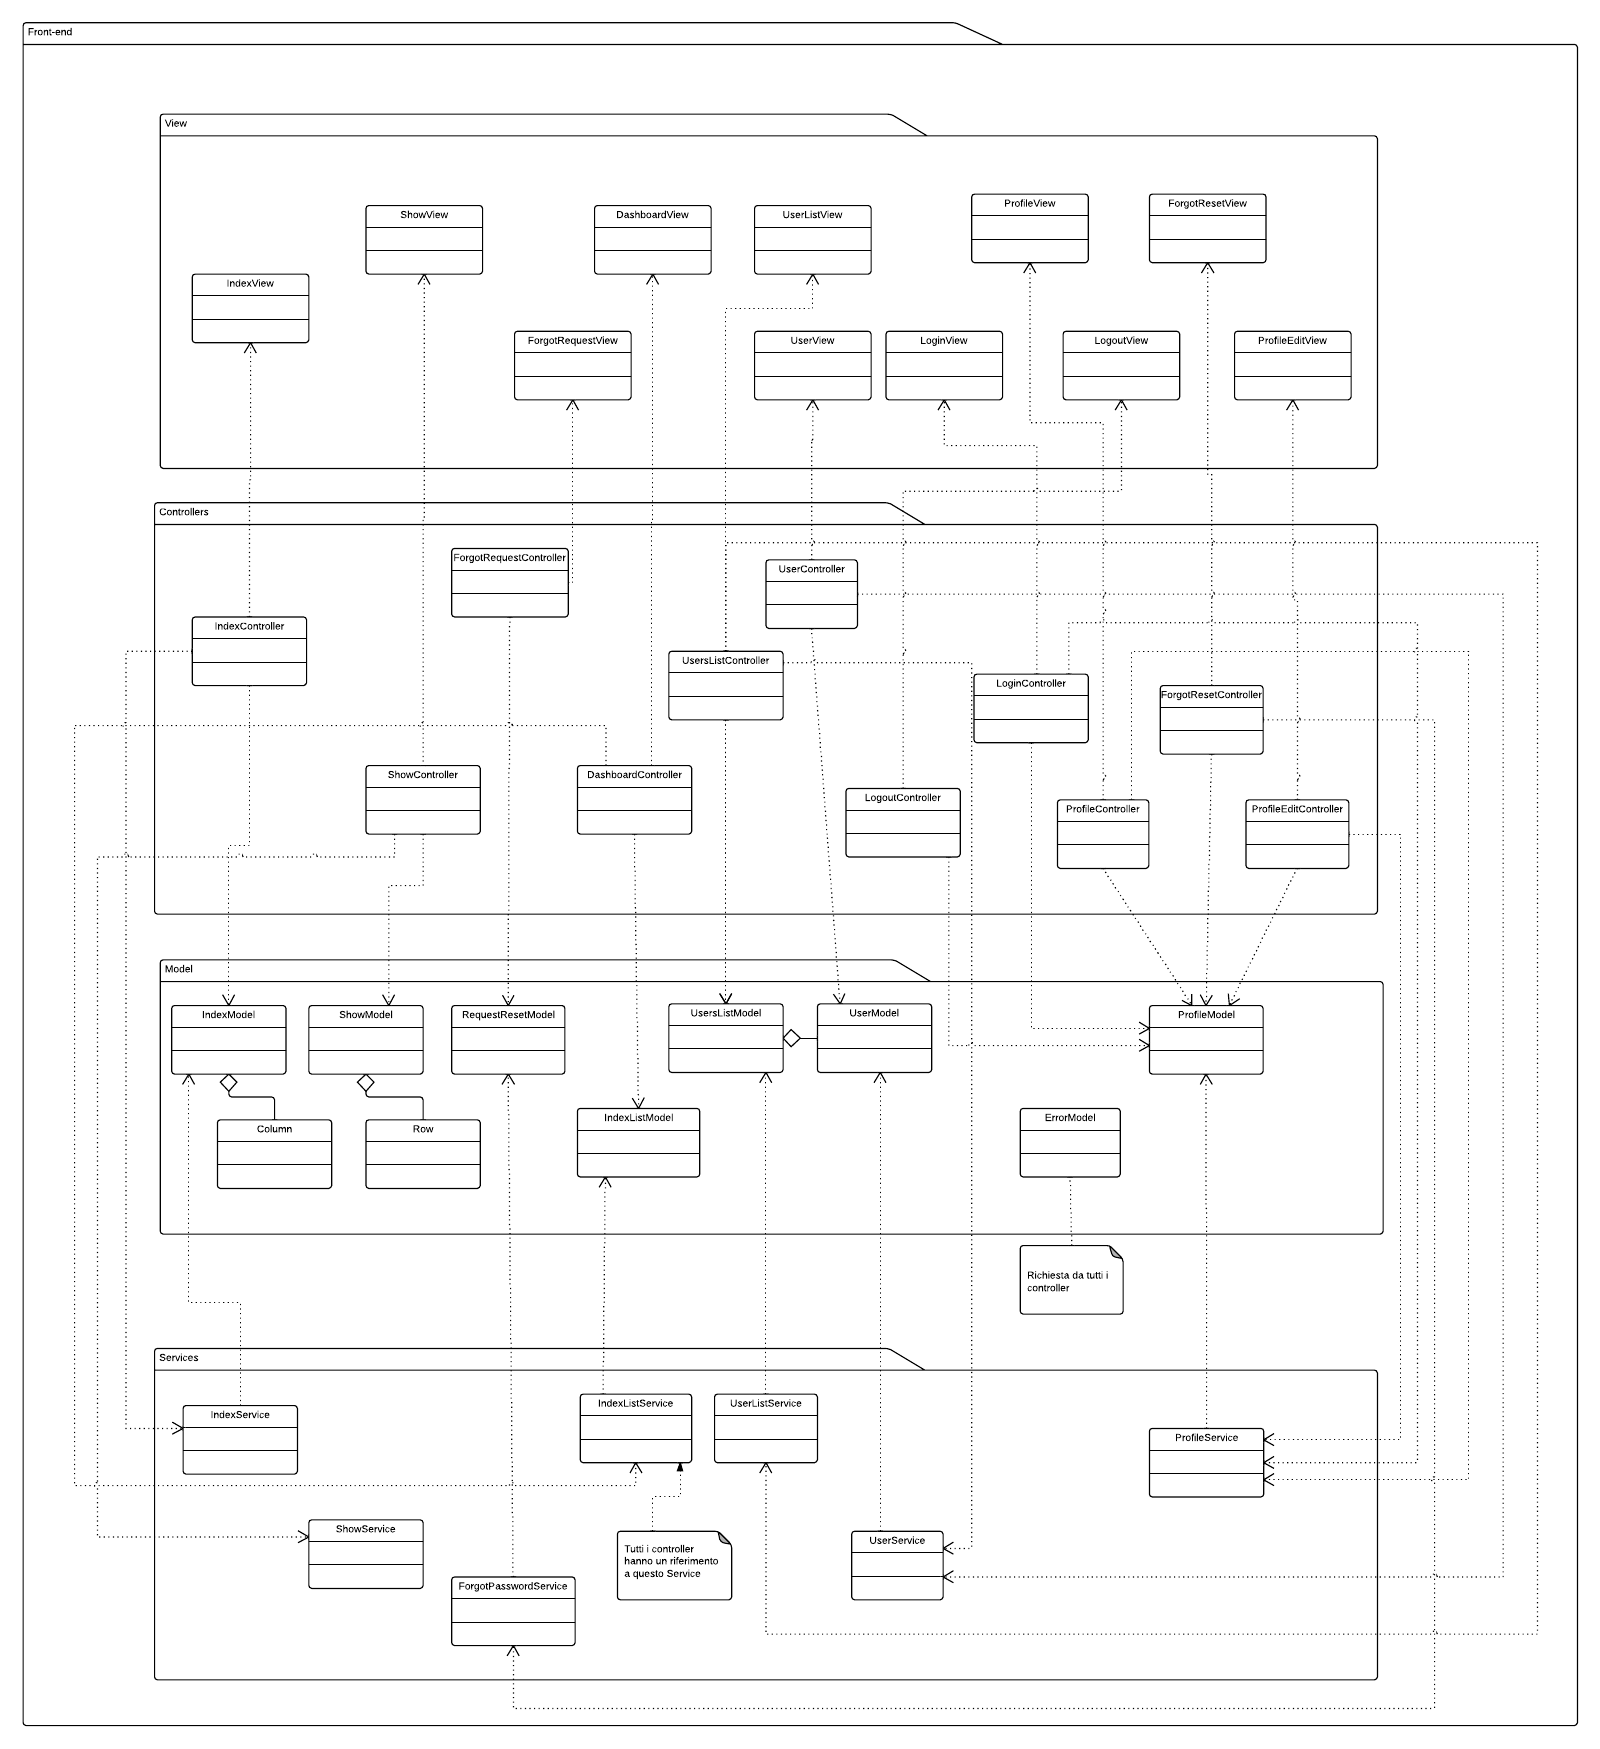
\includegraphics[width=\textwidth]{uml/classi/Front-end.png}  
        \caption{Diagramma delle classi Front-end}
      \end{center}  
    \end{figure} 
    
  \subparagraph{Descrizione} 
    \begin{itemize}
    \item[] \glossario{Package} che racchiude tutta la componente di \glossario{Front-end}. Comprende il sottosistema che viene eseguito nei browser degli utenti e che fornisce l'interfaccia grafica all'utente non-tecnico che utilizzerà l'applicazione.
    \end{itemize} 
    \subparagraph{Package contenuti} 
    \begin{itemize}
        \item Controllers
        \item Services
        \item Model
    \end{itemize}
  \subsubsection{Controllers}
  \paragraph{Informazioni sul package}
    \begin{figure}[H] 
      \begin{center}
        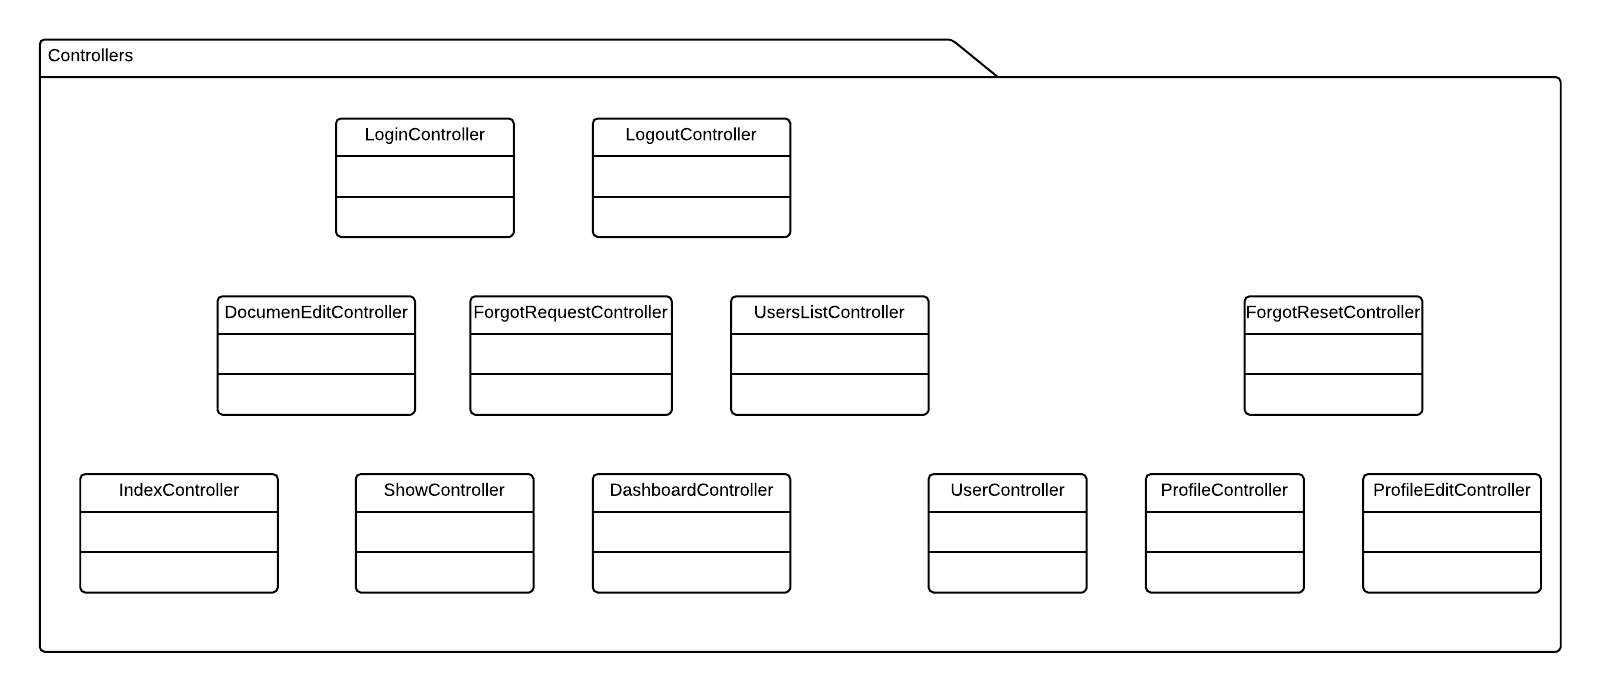
\includegraphics[width=\textwidth]{uml/package/Front-end::Controllers.png}
        \caption{Componente Controllers}
      \end{center}  
    \end{figure} 
  \subparagraph{Descrizione} 
    \begin{itemize}
    \item[] \glossario{Package} comprendente le classi che costituiscono i controller del componente \glossario{Front-end}. Ogni controller gestisce le operazioni e la logica applicativa riguardante una determinata pagina, e specifica quale view verrà utilizzata per la presentazione all'utente dei dati.
    \end{itemize} 
    \paragraph{Classi}
      \subparagraph{LoginController}
        
        \textbf{\\ \\ Descrizione} 
          \begin{itemize}
            \item[] Classe che gestisce le operazioni e la logica applicativa riguardante la pagina di Login.
          \end{itemize}      
        \textbf{Utilizzo}  
          \begin{itemize}
            \item[] Viene utilizzata per generare la pagina di login all'applicazione. Prima della creazione della view viene effettuato un controllo sull'esistenza di una sessione utente. In caso positivo il controller si occuperà di visualizzare una pagina nella quale l'utente verrà avvertito che un'autenticazione è già stata effettuata, altrimenti si procederà alla pagina di Login predefinita. Una volta che richiede un'autenticazione viene utilizzata classe \texttt{Front-End::Services::ProfileService}, la quale si occuperà di comunicare con il Back-End, il quale effettuerà il controllo sulle credenziali e in caso positivo effettuerà l'autenticazione dell'utente.
          \end{itemize}
      \subparagraph{LogoutController}
        
        \textbf{\\ \\ Descrizione} 
          \begin{itemize}
            \item[] Classe che gestisce l'operazione di logout di un utente.
          \end{itemize}      
        \textbf{Utilizzo}  
          \begin{itemize}
            \item[] Questa controller si occupa di distruggere la sessione attuale, se esiste, e non genera una view ma reindirizza l'utente automaticamente alla pagina di Login.
          \end{itemize}
      \subparagraph{ForgotResetController}
        
        \textbf{\\ \\ Descrizione} 
          \begin{itemize}
            \item[] Classe che gestisce le operazioni e la logica applicativa riguardante la pagina di reset della password.
          \end{itemize}      
        \textbf{Utilizzo}  
          \begin{itemize}
            \item[] Si occupa di generare la pagina di reset, prelevare quindi la nuova password inserita dall'utente nella view e chiamare l'apposito service che si occuperà del reset interagendo con il back-end.
          \end{itemize}
      \subparagraph{ProfileEditController}
        
        \textbf{\\ \\ Descrizione} 
          \begin{itemize}
            \item[] Classe che gestisce le operazioni di modifica di un utente attraverso la pagina profilo.
          \end{itemize}      
        \textbf{Utilizzo}  
          \begin{itemize}
            \item[] Utilizza la casse \texttt{Front-End::Services::ProfileService} per popolare la classe \texttt{Front-End::Model::ProfileModel} con i dati dell'utente. Quest'ultima classe fornirà un metodo accessorio attraverso il quale il controller può ottenere i dati e generare la pagina popolando correttamente lo scope.
          \end{itemize}
      \subparagraph{UserController}
        
        \textbf{\\ \\ Descrizione} 
          \begin{itemize}
            \item[] Classe che gestisce le operazioni e la logica applicativa riguardante la pagina profilo di un utente visualizzabile dall'admin.
          \end{itemize}      
        \textbf{Utilizzo}  
          \begin{itemize}
            \item[] Utilizza la classe \texttt{Front-End::Service::UserService}, che si occupa di popolare la classe \texttt{Front-End::Model::UserModel} con i dati dell'utente richiesto. Quest'ultima classe conterrà un metodo accessorio tramite il quale il controller può prelevare i dati e generare la pagina popolando correttamente lo scope.
          \end{itemize}
      \subparagraph{ProfileController}
        
        \textbf{\\ \\ Descrizione} 
          \begin{itemize}
            \item[] Classe che gestisce le operazioni e la logica applicativa riguardante la pagina profilo di un utente.
          \end{itemize}      
        \textbf{Utilizzo}  
          \begin{itemize}
            \item[] Utilizza la classe \texttt{Front-End::Services::ProfileService} per popolare la classe \texttt{Front-End::Model::ProfileModel} con i dati dell'utente che ha effettuato la richiesta. Quest'ultima classe fornirà un metodo accessorio attraverso il quale il controller potrà prelevare i dati e generare la pagina, popolando correttamente lo scope.
          \end{itemize}
      \subparagraph{ForgotRequestController}
        
        \textbf{\\ \\ Descrizione} 
          \begin{itemize}
            \item[] Classe che gestisce le operazioni e la logica applicativa riguardante la pagina di richiesta di recupero password.
          \end{itemize}      
        \textbf{Utilizzo}  
          \begin{itemize}
            \item[] Genera una pagina in cui viene visualizzato un campo di testo nel quale l'utente può inserire la propria mail ed effettuare una richiesta di ripristino password. Il controller permette quindi di inviare al Back-end la richiesta attraverso la classe \texttt{Front-End::Services::ForgotPasswordService}. Sarà poi compito del \glossario{Back-end} inviare all'utente una mail contenente il link che bisogna aprire per poter scegliere una nuova password.
          \end{itemize}
      \subparagraph{UsersListController}
        
        \textbf{\\ \\ Descrizione} 
          \begin{itemize}
            \item[] Classe che gestisce le operazioni e la logica applicativa riguardante la pagina di gestione degli utenti.
          \end{itemize}      
        \textbf{Utilizzo}  
          \begin{itemize}
            \item[] Viene utilizzata per generare la pagina di visualizzazione della lista di utenti presenti nell'applicazione. In primo luogo utilizzerà la classe \texttt{Front-End::Services::UserListService} per popolare la classe \texttt{Front-End::Model::UserListModel} dalla quale otterrà in seguito la lista degli utenti attraverso una chiamata a una sua funzione.
          \end{itemize}
      \subparagraph{CollectionController}
        
        \textbf{\\ \\ Descrizione} 
          \begin{itemize}
            \item[] Classe che gestisce le operazioni e la logica applicativa riguardante la pagina di gestione della Collection.
          \end{itemize}      
        \textbf{Utilizzo}  
          \begin{itemize}
            \item[] Utilizza la classe \texttt{Front-End::Services::CollectionService} per popolare correttamente la classe \texttt{Front-End::Model::CollectionModel}. Quest'ultima fornirà un metodo accessorio attraverso il quale il controller può ottenere i dati e generare la pagina di visualizzazione di tutti i \glossario{Document}, popolando correttamente lo scope.
          \end{itemize}
          \textbf{Relazioni con altre classi}
          \begin{itemize}
              \item{CollectionModel}
          \end{itemize}
      \subparagraph{DocumentEditController}
        
        \textbf{\\ \\ Descrizione} 
          \begin{itemize}
            \item[] Classe che gestisce le operazioni e la logica applicativa della pagina di modifica di un \glossario{Document}.
          \end{itemize}      
        \textbf{Utilizzo}  
          \begin{itemize}
            \item[] Utilizza la classe \texttt{Front-End::Services::DocumentService} per popolare correttamente la classe \texttt{Front-End::Model::DocumentModel} con i dati del \glossario{Document} richiesto. Quest'ultima classe fornirà un metodo accessorio attraverso il quale il controller potrà ottenere i dati e generare la pagina di modifica di un \glossario{Document} popolando correttamente lo scope.
          \end{itemize}
      \subparagraph{DashboardController}
        
        \textbf{\\ \\ Descrizione} 
          \begin{itemize}
            \item[] Classe che gestisce le operazioni e la logica applicativa riguardante la pagina dashboard.
          \end{itemize}      
        \textbf{Utilizzo}  
          \begin{itemize}
            \item[] Viene utilizzata per generare la pagina dashboard, che fungerà da \textit{home} dell'applicazione ovvero la prima pagina che un utente visualizza quando effettua l'autenticazione. Utilizza la classe \texttt{Front-End::Services::CollectionListService} per popolare correttamente tutte la classe \texttt{Front-End::Model::CollectionListModel}, dalla quale otterrà la lista delle \glossario{Collection} registrate nell'applicazione mediante una chiamata a una sua funzione. A questo punto, una volta ottenuti i dati, il controller genera la pagina dashboard, popolando correttamente lo scope con i dati ottenuti.
          \end{itemize}
      \subparagraph{DocumentController}
        
        \textbf{\\ \\ Descrizione} 
          \begin{itemize}
            \item[] Classe che gestisce le operazioni e la logica applicativa riguardante la pagina di gestione di un Document.
          \end{itemize}      
        \textbf{Utilizzo}  
          \begin{itemize}
            \item[] Utilizza la classe \texttt{Front-End::Services::DocumentService} per popolare correttamente la classe \texttt{Front-End::Model::DocumentModel}, la quale fornirà un metodo accessorio attraverso il quale il controller può ottenere i dati e generare la pagina popolando correttamente lo scope.
          \end{itemize}
  \subsubsection{Services}
  \paragraph{Informazioni sul package}
    \begin{figure}[H] 
      \begin{center}
        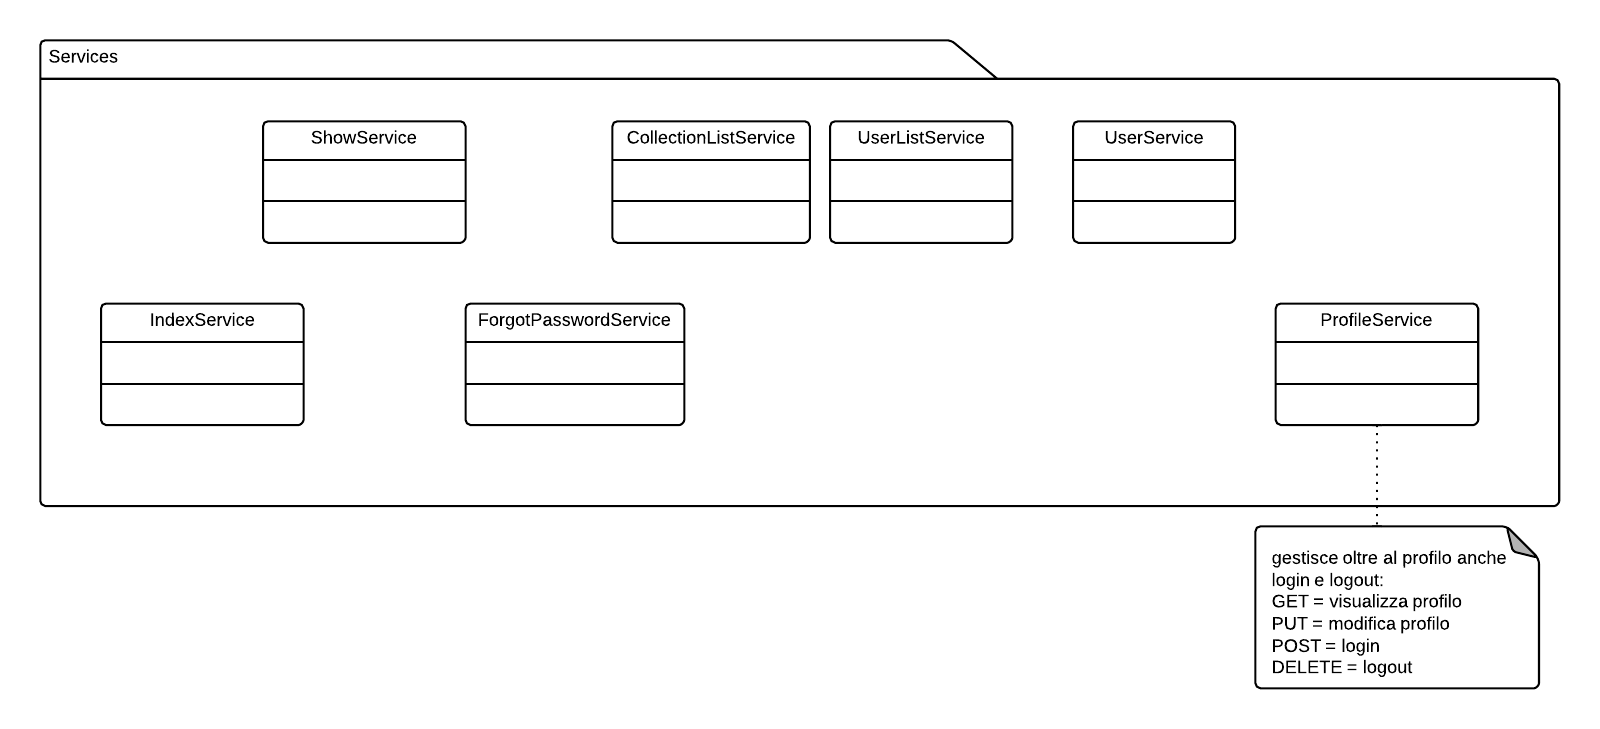
\includegraphics[width=\textwidth]{uml/package/Front-end::Services.png}
        \caption{Componente Services}
      \end{center}  
    \end{figure} 
  \subparagraph{Descrizione} 
    \begin{itemize}
    \item[] \glossario{Package} comprendente le classi che descrivono i meccanismi con cui il \glossario{Front-end} può interfacciarsi con le \glossario{API} del \glossario{Back-end}. Permette di recuperare i dati da inserire nel model e permette di azionare determinate procedure sul \glossario{Back-end} (per esempio la richiesta di recupero password o le ``action'' definite nel DSL).
    \end{itemize} 
    \paragraph{Classi}
      \subparagraph{ProfileService}
        
        \textbf{\\ \\ Descrizione} 
          \begin{itemize}
            \item[] Questa classe permette il recupero delle risorsa REST rappresentante il profilo utente tramite la chiamata /profile.
          \end{itemize}      
        \textbf{Utilizzo}  
          \begin{itemize}
            \item[] Le funzionalità offerte dalla classe sono:
\begin{itemize}
\item elenco dei dati relativi all'utente (GET);
\item modifica dei dati utente (PUT);
\item creazione della sessione utente (POST);
\item eliminazione della sessione utente (DELETE).
\end{itemize}

Per la funzionalità di visualizzazione dei dati, di modifica del profilo e di eliminazione della sessione è richiesto che l'utente sia autenticato.
          \end{itemize}
          \textbf{Relazioni con altre classi}
          \begin{itemize}
              \item{ProfileModel}
          \end{itemize}
      \subparagraph{UserListService}
        
        \textbf{\\ \\ Descrizione} 
          \begin{itemize}
            \item[] Questa classe permette il recupero delle risorse REST rappresentanti gli utenti registrati all'applicazione tramite la chiamata /users
          \end{itemize}      
        \textbf{Utilizzo}  
          \begin{itemize}
            \item[] La funzionalità offerta dalla classe è quella di poter fornire al Controller la lista degli utenti presenti nel database delle credenziali.
Tale funzionalità richiede che l'utente sia un admin.
          \end{itemize}
          \textbf{Relazioni con altre classi}
          \begin{itemize}
              \item{UsersListModel}
          \end{itemize}
      \subparagraph{CollectionListService}
        
        \textbf{\\ \\ Descrizione} 
          \begin{itemize}
            \item[] Questa classe permette il recupero delle risorse REST rappresentanti le Collections tramite la chiamata /collections
          \end{itemize}      
        \textbf{Utilizzo}  
          \begin{itemize}
            \item[] La funzionalità offerta dalla classe è quella di poter fornire al Controller la lista delle Collections registrate dallo sviluppatore e presenti nel database delle collections.
Tale funzionalità richiede che l'utente sia registrato.
          \end{itemize}
          \textbf{Relazioni con altre classi}
          \begin{itemize}
              \item{CollectionListModel}
          \end{itemize}
      \subparagraph{CollectionService}
        
        \textbf{\\ \\ Descrizione} 
          \begin{itemize}
            \item[] Questa classe permette il recupero della risorsa REST rappresentante la Collection tramite la chiamata  /collection/$\{$collection$\_$name$\}$
          \end{itemize}      
        \textbf{Utilizzo}  
          \begin{itemize}
            \item[] La  funzionalità offerta dalla classe è quella di poter fornire al Controller la lista di Document presenti nella Collection.
          \end{itemize}
      \subparagraph{DocumentService}
        
        \textbf{\\ \\ Descrizione} 
          \begin{itemize}
            \item[] Questa classe permette il recupero delle risorse REST rappresentanti i Document di una Collection tramite la chiamata /collections/$\{$collection$\_$name$\}$/$\{$document id$\}$
          \end{itemize}      
        \textbf{Utilizzo}  
          \begin{itemize}
            \item[] Le funzionalità offerte dalla classe sono: 
\begin{itemize} 
\item elenco dei dati relativi al Document 
\item modifica dei dati relativi al Document
\item rimozione del Document 
\end{itemize} 
Tali funzionalità richiedono che l'utente sia autenticato al sistema.
          \end{itemize}
          \textbf{Relazioni con altre classi}
          \begin{itemize}
              \item{DocumentModel}
          \end{itemize}
      \subparagraph{ForgotPasswordService}
        
        \textbf{\\ \\ Descrizione} 
          \begin{itemize}
            \item[] Questa classe si occupa di inviare al server una richiesta di recupero password tramite la chiamata /password/lost e la conseguente modifica attraverso la chiamata /password/reset.
          \end{itemize}      
        \textbf{Utilizzo}  
          \begin{itemize}
            \item[] La  funzionalità offerta dalla classe è quella di interagire col server delegando quest'ultimo all'invio di una mail all'utente per il recupero della password e successivamente alla sua modifica.
          \end{itemize}
          \textbf{Relazioni con altre classi}
          \begin{itemize}
              \item{RequestResetModel}
          \end{itemize}
      \subparagraph{UserService}
        
        \textbf{\\ \\ Descrizione} 
          \begin{itemize}
            \item[] Questa classe permette il recupero della risorsa REST rappresentante l'utente tramite la chiamata /users/$\{$user$\_$id$\}$
          \end{itemize}      
        \textbf{Utilizzo}  
          \begin{itemize}
            \item[] Le funzionalità offerte dalla classe sono: 
\begin{itemize} 
\item elenco dei dati relativi all'utente. 
\item modifica della password relativa al utente.
\item elevare o declassare un utente ad admin 
\item rimozione dell'utente.
\end{itemize}
Tali funzionalità richiedono che l'utente sia un admin.
          \end{itemize}
          \textbf{Relazioni con altre classi}
          \begin{itemize}
              \item{UserModel}
          \end{itemize}
  \subsubsection{Model}
  \paragraph{Informazioni sul package}
    \begin{figure}[H] 
      \begin{center}
        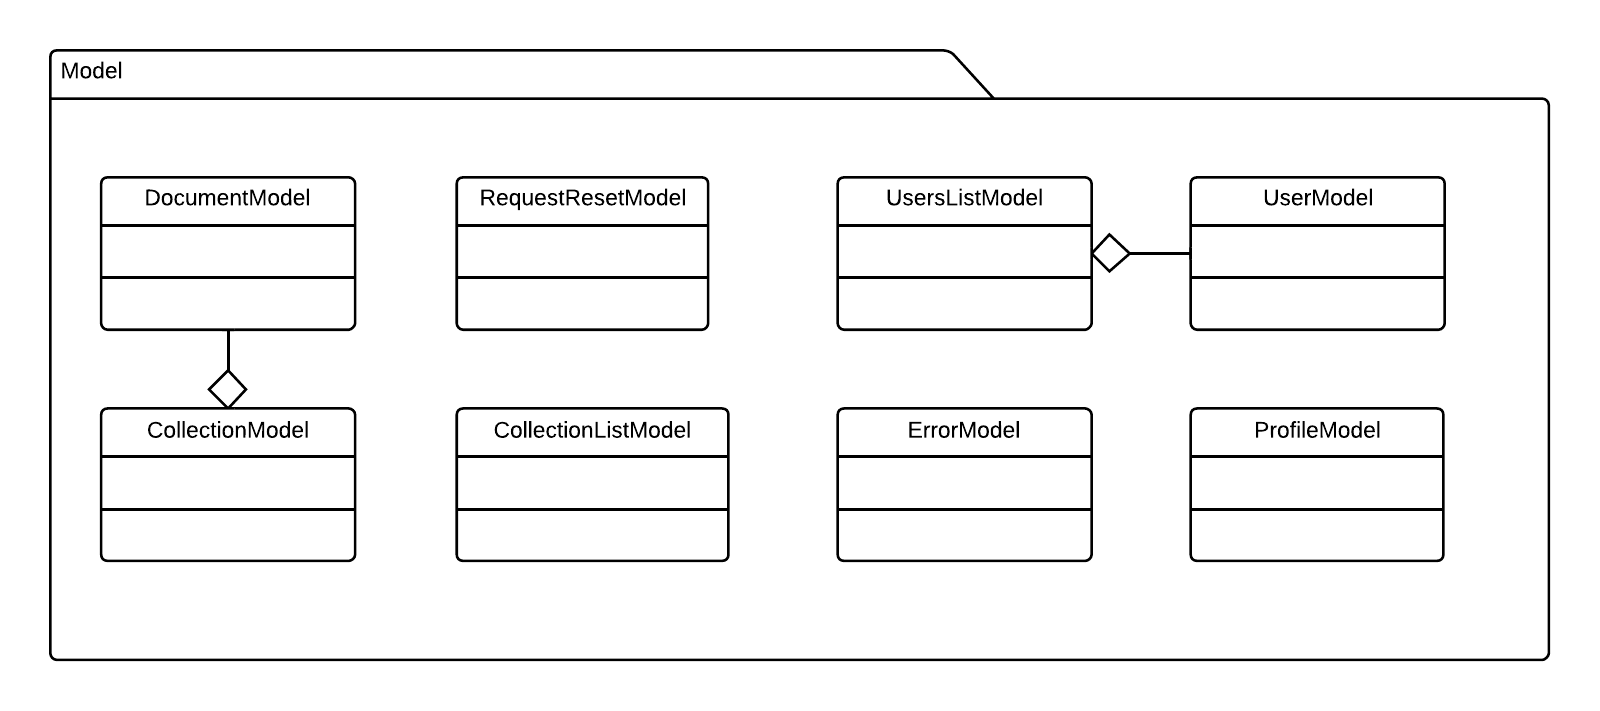
\includegraphics[width=\textwidth]{uml/package/Front-end::Model.png}
        \caption{Componente Model}
      \end{center}  
    \end{figure} 
  \subparagraph{Descrizione} 
    \begin{itemize}
    \item[] \glossario{Package} che comprende le classi dei modelli dei dati utilizzati dal \glossario{Front-end}. Servono a fornire ai controller e ai service le informazioni su quali campi potranno aspettarsi negli oggetti che arrivano tramite le \glossario{API} del \glossario{Back-end}.

Le classi di questo \glossario{package} sono state progettate, ma si prevede che non verranno codificate poiché verrà sfruttato lo stile di \glossario{duck-typing} della gestione dei tipi di \glossario{JavaScript}.
    \end{itemize} 
    \paragraph{Classi}
      \subparagraph{ErrorModel}
        
        \textbf{\\ \\ Descrizione} 
          \begin{itemize}
            \item[] È la classe che rappresenta il modello dati dell'errore.
          \end{itemize}      
        \textbf{Utilizzo}  
          \begin{itemize}
            \item[] Utilizzato da tutti i controller per poter accedere alle informazioni riguardanti l'errore.
          \end{itemize}
      \subparagraph{CollectionListModel}
        
        \textbf{\\ \\ Descrizione} 
          \begin{itemize}
            \item[] È la classe che rappresenta la struttura dati delle Collections.
          \end{itemize}      
        \textbf{Utilizzo}  
          \begin{itemize}
            \item[] Fornisce una rappresentazione sotto forma di oggetto delle informazioni scambiate con il back-end e permette alla CollectionListService e alla DashboardController di poter accedere alla lista delle Collections.
          \end{itemize}
      \subparagraph{UserModel}
        
        \textbf{\\ \\ Descrizione} 
          \begin{itemize}
            \item[] È la classe che rappresenta la struttura dati dell'utente.
          \end{itemize}      
        \textbf{Utilizzo}  
          \begin{itemize}
            \item[] Fornisce una rappresentazione sotto forma di oggetto delle informazioni scambiate con il back-end e permette allo UserService e allo UserController di poter accedere agli attributi dell'utente.
          \end{itemize}
      \subparagraph{RequestResetModel}
        
        \textbf{\\ \\ Descrizione} 
          \begin{itemize}
            \item[] È il modello che contiene i dati dell'utente che richiede un recupero della password.
          \end{itemize}      
        \textbf{Utilizzo}  
          \begin{itemize}
            \item[] Fornisce una rappresentazione sotto forma di oggetto delle informazioni scambiate con il back-end e permette al ForgotPasswordService e al ForgotRequestController di poter accedere ai dati dell'utente.
          \end{itemize}
      \subparagraph{DocumentModel}
        
        \textbf{\\ \\ Descrizione} 
          \begin{itemize}
            \item[] È la classe che rappresenta la struttura dati dei Document relativi ad una Collection.
          \end{itemize}      
        \textbf{Utilizzo}  
          \begin{itemize}
            \item[] Fornisce una rappresentazione sotto forma di oggetto delle informazioni scambiate con il back-end e permette al DocumentService e al DocumentController di poter accedere agli attributi del Document.
          \end{itemize}
      \subparagraph{ProfileModel}
        
        \textbf{\\ \\ Descrizione} 
          \begin{itemize}
            \item[] È la classe che rappresenta la struttura dati dell'utente.
          \end{itemize}      
        \textbf{Utilizzo}  
          \begin{itemize}
            \item[] Permette al ProfileService di avere una rappresentazione delle informazioni dell'utente da scambiare con il back-end, al ProfileController e al ProfileEditController per ottenere il dati dell'utente da visualizzare nella view della pagina profilo e al ForgotResetController per la modifica della password.
          \end{itemize}
      \subparagraph{CollectionModel}
        
        \textbf{\\ \\ Descrizione} 
          \begin{itemize}
            \item[] È la classe che rappresenta il modello delle Collection.
          \end{itemize}      
        \textbf{Utilizzo}  
          \begin{itemize}
            \item[] Fornisce una rappresentazione sotto forma di oggetto delle informazioni scambiate con il back-end e permette alla CollectionService e alla CollectionController di poter accedere alla lista delle Collections.
          \end{itemize}
      \subparagraph{UsersListModel}
        
        \textbf{\\ \\ Descrizione} 
          \begin{itemize}
            \item[] È la classe che rappresenta la struttura dati dell'utente.
          \end{itemize}      
        \textbf{Utilizzo}  
          \begin{itemize}
            \item[] Fornisce una rappresentazione sotto forma di oggetto delle informazioni scambiate con il back-end e permette allo UserListService e allo UserListController di poter accedere alla lista degli utenti.
          \end{itemize}